\documentclass[12pt,a4paper,onecolumn]{article}
\title{\Large{\textit{Pregancy Infomations}}}
\author{WuXiaochun}

\date{}

\usepackage{fontspec,xunicode,xltxtra}
% \setmainfont[Mapping=tex-text]{Times New Roman}
\setmainfont[Mapping=tex-text]{Arial}
\setsansfont[Mapping=tex-text]{Arial}
% \setmonofont[Mapping=tex-text]{Courier New}
\setmonofont[Mapping=tex-text]{Times New Roman}

\usepackage{xeCJK}
% \setCJKmainfont[ItalicFont={Adobe Kaiti Std}]{Adobe Song Std}
% \setCJKmainfont[ItalicFont={Adobe Kaiti Std}]{Adobe Kaiti Std}
\setCJKmainfont[ItalicFont={Adobe Kaiti Std}]{Adobe Heiti Std}
\setCJKsansfont{Adobe Heiti Std}
% \setCJKsansfont{Microsoft YaHei}
\setCJKmonofont{Adobe Heiti Std}
\punctstyle{banjiao}

\usepackage{calc}
\usepackage[]{geometry}
% \geometry{paperwidth=221mm,paperheight=148.5mm}
% \geometry{paperwidth=9.309in,paperheight=6.982in}
\geometry{paperwidth=7.2cm,paperheight=10.8cm}
% \geometry{twocolumn}
\geometry{left=5mm,right=5mm}
\geometry{top=5mm,bottom=5mm,foot=5mm}
% \geometry{columnsep=10mm}
\setlength{\emergencystretch}{3em}


\usepackage{indentfirst}

%生成PDF的链接
\usepackage{hyperref}
\hypersetup{
    % bookmarks=true,         % show bookmarks bar?
    bookmarksopen=true,
    pdfpagemode=UseNone,    % options: UseNode, UseThumbs, UseOutlines, FullScreen
    pdfstartview=FitB,
    pdfborder=1,
    pdfhighlight=/P,
    pdfauthor={wuxch},
    unicode=true,           % non-Latin characters in Acrobat’s bookmarks
    colorlinks,             % false: boxed links; true: colored links
    linkcolor=blue,         % color of internal links
    citecolor=blue,        % color of links to bibliography
    filecolor=magenta,      % color of file links
    urlcolor=cyan           % color of external links
}
\makeindex

\usepackage[dvips,dvipsnames,svgnames]{xcolor}
\definecolor{light-gray}{gray}{0.95}

\usepackage{graphicx}
\usepackage{wrapfig}
\usepackage{picinpar}

\renewcommand\contentsname{目录}
\renewcommand\listfigurename{插图}
\renewcommand\listtablename{表格}
\renewcommand\indexname{索引}
\renewcommand\figurename{图}
\renewcommand\tablename{表}

\usepackage{caption}
\renewcommand{\captionfont}{\scriptsize \sffamily}
\setlength{\abovecaptionskip}{0pt}
\setlength{\belowcaptionskip}{0pt}

\graphicspath{{fig/}}

\usepackage{fancyhdr}

% \usepackage{lastpage}
% \cfoot{\thepage\ of \pageref{LastPage}}

% 嵌入的代码显示
% \usepackage{listings}
% \lstset{language=C++, breaklines, extendedchars=false}
% \lstset{basicstyle=\ttfamily,
%         frame=single,
%         keywordstyle=\color{blue},
%         commentstyle=\color{SeaGreen},
%         stringstyle=\ttfamily,
%         showstringspaces=false,
%         tabsize=4,
%         backgroundcolor=\color{light-gray}}

\usepackage[sf]{titlesec}
\titleformat{\section}{\normalsize\sffamily\bf\color{blue}}{\textsection~\thesection}{.1em}{}
\titleformat{\subsection}{\normalsize\sffamily}{\thesubsection}{.1em}{}
\titlespacing*{\section}{0pt}{1ex}{1ex}
\titlespacing*{\subsection}{0pt}{0.2ex}{0.2ex}

\usepackage{fancyhdr}
\usepackage{lastpage}
\fancyhf{}
\lhead{}
\rhead{}
\chead{\scriptsize{\textsf{蜗居}}}
\cfoot{\scriptsize{\textsf{第 \thepage ~页,共 \pageref*{LastPage} 页}}}


% \usepackage{enumitem}
% \setitemize{label=$\bullet$,leftmargin=3em,noitemsep,topsep=0pt,parsep=0pt}
% \setenumerate{leftmargin=3em,noitemsep,topsep=0pt,parsep=0pt}

% \setlength{\parskip}{1.5ex plus 0.5ex minus 0.2ex}
\setlength{\parskip}{2.0ex plus 0.5ex minus 0.2ex}

% \setlength{\parindent}{5ex}
\setlength{\parindent}{0ex}

% \usepackage{setspace}
\linespread{1.25}

% 英文的破折号--不明显,使用自己画的线。
\newcommand{\myrule}{\hspace{0.5em}\rule[3pt]{1.6em}{0.3mm}\hspace{0.5em}}


\begin{document}

\maketitle

\thispagestyle{empty}
\pagebreak

\thispagestyle{empty}
\vfill
\vfill

\begin{center}
{\large {\it To my sweety wife and brilliant unborn child.}}
\end{center}
\vfill
\pagebreak

\setcounter{page}{1}
\pagenumbering{roman}
\pagestyle{plain}
\tableofcontents
\pagebreak
\listoffigures
\pagebreak
\setcounter{page}{1}
\pagenumbering{arabic}
\pagestyle{fancy}
\section{General Conception}

\begin{figwindow}[0,r,{\mbox{\includegraphics[width=0.25\textwidth]{Expecting_mother.jpg}}},A
  pregnant woman near the end of her term]
  \textbf{Pregnancy} (latin graviditas) is the carrying of one or more offspring, known as a fetus
  or embryo, inside the uterus of a female. In a pregnancy, there can be multiple gestations, as in
  the case of twins or triplets. Human pregnancy is the most studied of all mammalian pregnancies.
  Obstetrics is the surgical field that studies and cares for high risk pregnancy. Midwifery is the
  non-surgical field that cares for pregnancy and pregnant women.


Childbirth usually occurs about 38 weeks after fertilization (conception), i.e., approximately 40
weeks from the last normal menstrual period (LNMP) in humans. The World Health Organisation defines
normal term for delivery as between 37 weeks and 42 weeks. The calculation of this date involves the
assumption of a regular 28-day period.

\end{figwindow}

\section{Terminology}

One scientific term for the state of pregnancy is gravid, and a pregnant female is sometimes
referred to as a gravida. Neither word is used in common speech. Similarly, the term "parity"
(abbreviated as "para") is used for the number of previous successful live births. Medically, a
woman who has never been pregnant is referred to as a "nulligravida", and in subsequent pregnancies
as "multigravida" or "multiparous". Hence during a second pregnancy a woman would be described as
"gravida 2, para 1" and upon delivery as "gravida 2, para 2". Incomplete pregnancies of abortions,
miscarriages or stillbirths account for parity values being less than the gravida number, whereas a
multiple birth will increase the parity value. Women who have never carried a pregnancy achieving
more than 20 weeks of gestation age are referred to as "nulliparous". The medical term for a woman
who is pregnant for the first time is primipara.

The term embryo is used to describe the developing offspring during the first eight weeks following
conception, and the term fetus is used from about two months of development until birth.

In many societies' medical or legal definitions, human pregnancy is somewhat arbitrarily divided
into three trimester periods, as a means to simplify reference to the different stages of prenatal
development. The first trimester carries the highest risk of miscarriage (natural death of embryo or
fetus). During the second trimester, the development of the fetus can be more easily monitored and
diagnosed. The beginning of the third trimester often approximates the point of viability, or the
ability of the fetus to survive, with or without medical help, outside of the uterus.

\section{Progression}

\subsection{Initiation}

Pregnancy occurs as the result of the female gamete or oocyte being penetrated by the male gamete
spermatozoon in a process referred to, in medicine, as "fertilization", or more commonly known as
"conception". After the point of "fertilization" it is referred to as an egg. The fusion of male and
female gametes usually occurs through the act of sexual intercourse. However, the advent of
artificial insemination and in vitro fertilisation have also made achieving pregnancy possible in
cases where sexual intercourse does not result in fertilization (e.g. through choice or male/female
infertility).

\subsection{Prenatal period}

\textbf{Prenatal} or \textbf{antenatal development} is the process in which an embryo or fetus (or
foetus) gestates during pregnancy, from fertilization until birth. Often, the terms \textbf{fetal
  development}, \textbf{foetal development}, or \textbf{embryology} are used in a similar sense.

After fertilization the embryogenesis starts. In humans, when embryogenesis finishes, by the end of
the 10th week of gestational age, the precursors of all the major organs of the body have been
created. Therefore, the following period, the fetal period, is described both topically on one hand,
i.e. by organ, and strictly chronologically on the other, by a list of major occurrences by weeks of
gestational age.

\subsubsection{Fertilization}

\begin{figwindow}[0,r,{\mbox{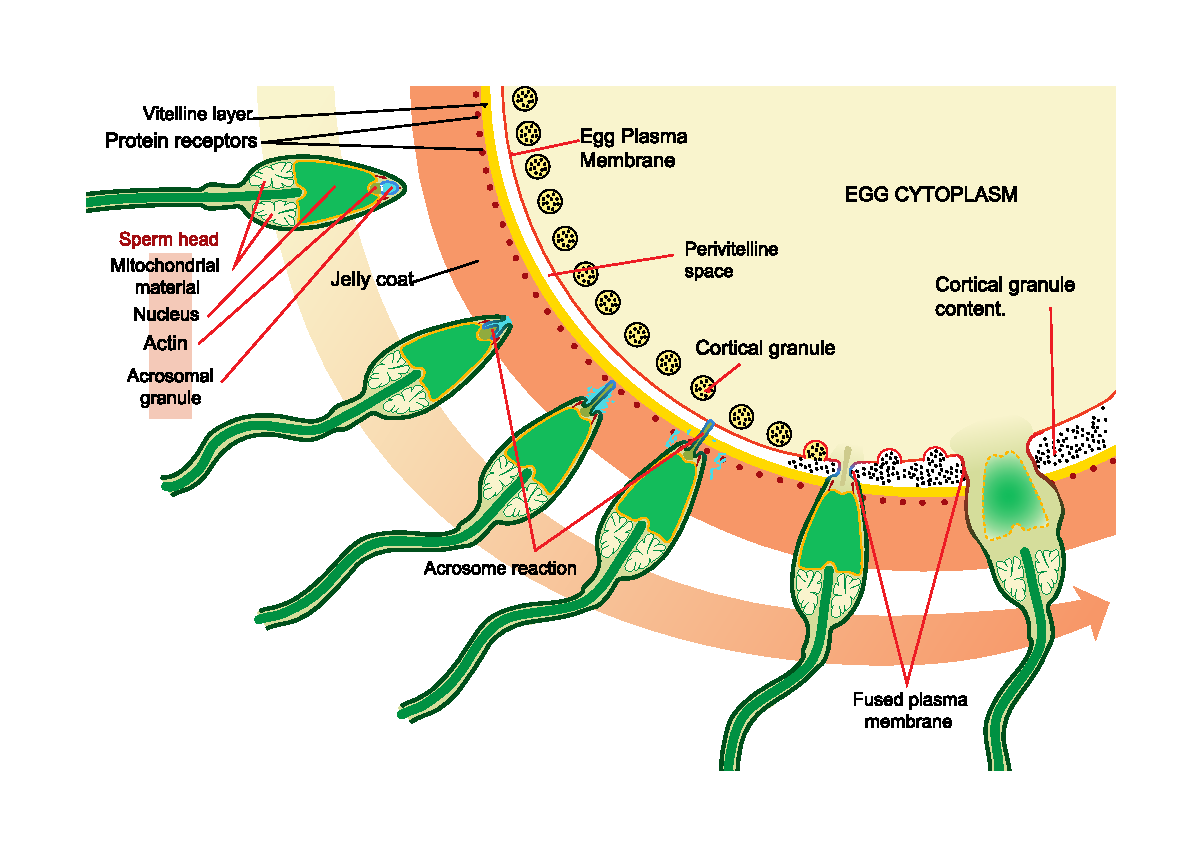
\includegraphics[width=0.5\textwidth]{Acrosome_reaction_diagram}}},A sperm
  fertilizing an ovum]
When semen is deposited in the vagina, the spermatozoa travel through the cervix and body of the
uterus and into the Fallopian tubes. Fertilization of the ovum (egg cell) usually takes place in the
Fallopian tube. Many sperm must cooperate to penetrate the thick protective shell-like barrier that
surrounds the ovum. The first sperm that penetrates fully into the egg donates its genetic material
(DNA). The egg then polarizes, repelling any additional sperm. The resulting combination is called a
zygote. The term "conception" refers variably to either fertilization or to formation of the
conceptus after uterine implantation, and this terminology is controversial.
\end{figwindow}

Prior to fertilization, each ovum contains a complete human genome, including a single X but no Y
chromosome. Likewise, each spermatozoon contains a complete set of autosomes and a single sex
chromosome, either X or Y. The resulting zygote is similar to the majority of somatic cells because
it contains two copies of the genome in a diploid set of chromosomes. One set of chromosomes came
from the nucleus of the ovum and the second set from the nucleus of the sperm. If the spermatozoon
contributes a Y chromosome then the zygote will develop as a male. Unlike the X chromosome, the Y
chromosome contains very little genetic information. However it does contain a gene, SRY, which will
switch on androgen production at a later stage, leading to the development of a male body type. In
contrast, the mitochondrial genetic information of the zygote comes entirely from the mother via the
ovum.


\subsubsection{Embryonic period}

The embryonic period in humans begins at fertilization (2nd week of gestation) and continues until
the end of the 10th week of gestation (8th week of development).

The zygote spends the next few days traveling down the Fallopian tube. Meanwhile it divides several
times to form a ball of cells called a morula. Further cellular division is accompanied by the
formation of a small cavity between the cells. This stage is called a blastocyst. Up to this point
there is no growth in the overall size of the embryo, so each division produces successively smaller
cells.

The blastocyst reaches the uterus at roughly the fifth day after fertilization. It is here that
lysis of the zona pellucida, a glycoprotein shell, occurs. This is required so that the
trophectoderm cells, which give rise to extra-embryonic structures such as the placenta, of the
blastocyst can come into contact with the luminal epithelial cells of the endometrium. (Contrast
this with zona hatching, an event that occurs in vitro by a different mechanism, but with a similar
result). It then adheres to the uterine lining and becomes embedded in the endometrial cell layer.
This process is also called implantation. In most successful pregnancies, the conceptus implants 8
to 10 days after ovulation (Wilcox et al. 1999). The inner cell mass forms the embryo, while the
outer cell layers form the membranes and placenta. Together, the embryo and its membranes are
referred to as a conceptus, or the ``products of conception''.

Rapid growth occurs and the embryo's main external features begin to take form. This process is
called differentiation, which produces the varied cell types (such as blood cells, kidney cells, and
nerve cells). A spontaneous abortion, or miscarriage, in the first trimester of pregnancy is usually
due to major genetic mistakes or abnormalities in the developing embryo. During this critical period
(most of the first trimester), the developing embryo is also susceptible to toxic exposures, such
as:
\begin{wuxch_item}
    \item Alcohol, certain drugs, and other toxins that cause birth defects, such as Fetal alcohol syndrome
    \item Infection (such as rubella or cytomegalovirus)
    \item Radiation from x-rays or radiation therapy
    \item Nutritional deficiencies such as lack of folate which contributes to spina bifida
\end{wuxch_item}

Generally, if a structure pre-dates another structure in evolutionary terms, then it often appears
earlier than the other in an embryo; this general observation is sometimes summarized by the phrase
``ontogeny recapitulates phylogeny.'' For example, the backbone is a common structure among all
vertebrates such as fish, reptiles and mammals, and the backbone also appears as one of the earliest
structures laid out in all vertebrate embryos. The cerebrum in humans, which is the most
sophisticated part of the brain, develops last. The concept of recapitulation is not absolute, but
it is recognized as being partly applicable to development of the human embryo.

\subsubsection{Changes by weeks of gestation}

\subsubsection{Gestational age vs. embryonic age}

Gestational age is the time that has passed since the onset of the last menstruation, which
generally or as standard occurs 2 weeks before the actual fertilization. Embryonic age, in contrast
measures the actual age of the embryo or fetus from the time of fertilization. Nevertheless,
menstruation has historically been the only means of estimating embryonal/fetal age, and is still
the presumed measure if not else specified.

Thus, the first week of embryonic age is already week three counting with gestational age. The other
way around, week 1 and 2 of gestational age are merely theoretical extrapolations of embryonic age,
since the embryo actually hasn't yet formed.

Furthermore, the number of the week is one more than the actual age of the embryo/fetus. For
example, the embryo is 0 whole weeks old during the 1st week after fertilization.

The following table summarizes the various expression systems during week number x of gestation.
\begin{table}
\begin{center}
\begin{tabular}{ccc}
  \hline
  \textbf{Week} & number & reached age \\
  \hline
  \textbf{Gestational} & x & x-1 \\
  \textbf{Embryonic} & x-2 & x-3 \\
  \hline
\end{tabular}
\end{center}
\end{table}

\subsubsection{Week 3}

Gestational age: 2 weeks old. 15-21 days from last menstruation.

Embryonic age: Week nr 1. 0 weeks old. 1-7 days from fertilization.

\begin{wuxch_item}
    \item Fertilization of the ovum to form a zygote. (day 1 of fert.)
    \item The zygote undergoes mitotic cellular divisions, but does not increase in size. This
      mitosis is also known as cleavage. A hollow cavity forms marking the blastocyst stage. (day
      1.5-3 of fert.)
    \item The blastocyst contains only a thin rim of trophoblast cells and a clump of cells at
      one end known as the ``embryonic pole'' which include embryonic stem cells.
    \item The embryo hatches from its protein shell (zona pellucida) and performs implantation
      onto the endometrial lining of the mother's uterus. (day 5-6 of fert.)
    \item If separation into identical twins occurs, 1/3 of the time it will happen before day 5.
\end{wuxch_item}

\subsubsection{Week 4}

Gestational age: 3 weeks old. 22-28 days from last menstruation.

Embryonic age: Week nr 2. 1 week old. 8-14 days from fertilization.

\begin{wuxch_item}
    \item rophoblast cells surrounding the embryonic cells proliferate and invade deeper into the
  uterine lining. They will eventually form the placenta and embryonic membranes. The blastocyst is
  fully implanted day 7-12 of fert.
    \item Formation of the yolk sac.
    \item The embryonic cells flatten into a disk, two cells thick.
    \item If separation into identical twins occurs, 2/3 of the time it will happen between days 5
      and 9. If it happens after day 9, there is a significant risk of the twins being conjoined.
    \item Primitive streak develops. (day 13 of fert.)
    \item Primary stem villi appear. (day 13 of fert.)
\end{wuxch_item}

\subsubsection{Week 5}

Gestational age: 4 weeks old. 29-35 days from last menstruation.

Embryonic age: Week nr 3. 2 weeks old. 15-21 days from fertilization.

\begin{wuxch_item}
    \item A notochord forms in the center of the embryonic disk. (day 16 of fert.)
    \item Gastrulation commences. (day 16 of fert.)
    \item A neural groove (future spinal cord) forms over the notochord with a brain bulge at one end. Neuromeres appear. (day 18 of fert.)
    \item Somites, the divisions of the future vertebra, form. (day 20 of fert.)
    \item Primitive heart tube is forming. Vasculature begins to develop in embryonic disc. (day 20 of fert.)
\end{wuxch_item}

\subsubsection{Week 6}

Gestational age: 5 weeks old. 36-42 days from last menstruation.

Embryonic age: Week nr 4. 3 weeks old. 22-28 days from fertilization.

\begin{wuxch_item}
    \item The embryo measures 4 mm (1/8 inch) in length and begins to curve into a C shape.
    \item The heart bulges, further develops, and begins to beat in a regular rhythm. Septum primum appear.
    \item Branchial arches, grooves which will form structures of the face and neck, form.
    \item The neural tube closes.
    \item The ears begin to form as otic pits.
    \item Arm buds and a tail are visible.
    \item Pulmonary primordium, the first traits of the lung appear.
    \item Hepatic plate, the first traits of the liver appear.
    \item Buccopharyngeal membrane ruptures. This is the future mouth.
    \item Cystic diverticulum, which will become the gallbladder, and dorsal pancreatic bud, which
      will become the pancreas appear.
    \item Urorectal septum begins to form. Thus, the rectal and urinary passageways become separated.
    \item Anterior and posterior horns differentiate in the spinal cord
    \item Spleen appears.
    \item Ureteric buds appear.
\end{wuxch_item}

\subsubsection{Week 7}

Gestational age: 6 weeks old. 43-49 days from last menstruation.

Embryonic age: Week nr 5. 4 weeks old. 29-35 days from fertilization.

\begin{wuxch_item}
    \item The embryo measures 8 mm (1/4 inch) in length.
    \item Lens pits and optic cups form the start of the developing eye.
    \item Nasal pits form.
    \item The brain divides into 5 vesicles, including the early telencephalon.
    \item Leg buds form and hands form as flat paddles on the arms.
    \item Rudimentary blood moves through primitive vessels connecting to the yolk sac and chorionic membranes.
\end{wuxch_item}

\subsubsection{Week 8}

Gestational age: 7 weeks old. 50-56 days from last menstruation.

Embryonic age: Week nr 6. 5 weeks old. 36-42 days from fertilization.

\begin{wuxch_item}
    \item The embryo measures 13 mm (1/2 inch) in length.
    \item Lungs begin to form.
    \item The brain continues to develop.
    \item Arms and legs have lengthened with foot and hand areas distinguishable.
    \item The hands and feet have digits, but may still be webbed.
    \item The gonadal ridge begins to be perceptible.
    \item The lymphatic system begins to develop.
\end{wuxch_item}

\subsubsection{Week 9}

Gestational age: 8 weeks old. 57-63 days from last menstruation.

Embryonic age: Week nr 7. 6 weeks old. 43-49 days from fertilization.

\begin{wuxch_item}
    \item The embryo measures 18 mm (3/4 inch) in length.
    \item Nipples and hair follicles begin to form.
    \item Location of the elbows and toes are visible.
    \item Spontaneous limb movements may be detected by ultrasound.
    \item All essential organs have at least begun formation.
\end{wuxch_item}

\subsubsection{Fetal period}

The fetal period begins at the end of the 10th week of gestation (8th week of development). Since
the precursors of all the major organs are created by this time, the fetal period is described both
by organ and by a list of changes by weeks of gestational age.

Because the precursors of the organs are formed, fetus also is not as sensitive to damage from
environmental exposures as the embryo. Instead, toxic exposures often cause physiological
abnormalities or minor congenital malformation.

\subsubsection{Changes by weeks of gestation}

From the 8th week until birth (around 38 weeks), the developing organism is called a fetus. The
fetus is not as sensitive to damage from environmental exposures as the embryo, and toxic exposures
often cause physiological abnormalities or minor congenital malformation. All major structures are
already formed in the fetus, but they continue to grow and develop.

\subsubsection{Weeks 10-12}

Gestational age: 9-11 weeks old.

Embryonic age: Weeks nr 8-10. 7-9 weeks old.

\begin{wuxch_item}
    \item Embryo measures 30 mm-8 cm (1.2-3.2 inches) in length.
    \item Intestines rotate.
    \item Facial features continue to develop.
    \item the eyelids are more developed.
    \item the external features of the ear begin to take their final shape.
    \item The head comprises nearly half of the fetus' size.
    \item The face is well formed
    \item The eyelids close and will not reopen until about the 28th week.
    \item Tooth buds, which will form the baby teeth, appear.
    \item The limbs are long and thin.
    \item The fetus can make a fist with its fingers.
    \item Genitals appear well differentiated.
    \item Red blood cells are produced in the liver.
\end{wuxch_item}

\subsubsection{Weeks 13 to 16}

Gestational age: 12-15 weeks old.

Embryonic age: Weeks nr 11-14. 10-13 weeks old.
\begin{wuxch_item}
    \item The fetus reaches a length of about 15 cm (6 inches).
    \item A fine hair called lanugo develops on the head.
    \item Fetal skin is almost transparent.
    \item More muscle tissue and bones have developed, and the bones become harder.
    \item The fetus makes active movements.
    \item Sucking motions are made with the mouth.
    \item Meconium is made in the intestinal tract.
    \item The liver and pancreas produce fluid secretions.
\end{wuxch_item}

\subsubsection{Week 19}

Gestational age: 18 weeks old.

Embryonic age: Week nr 17. 16 weeks old.

\begin{wuxch_item}
    \item The fetus reaches a length of 20 cm (8 inches).
    \item Lanugo covers the entire body.
    \item Eyebrows and eyelashes appear.
    \item Nails appear on fingers and toes.
    \item The fetus is more active with increased muscle development.
    \item "Quickening" usually occurs (the mother can feel the fetus moving).
    \item The fetal heartbeat can be heard with a stethoscope.
\end{wuxch_item}

\subsubsection{Week 23}

Gestational age: 22 weeks old.

Embryonic age: Week nr 21. 20 weeks old.
\begin{wuxch_item}
    \item The fetus reaches a length of 28 cm (11.2 inches).
    \item The fetus weighs about 725 g (1 lb 10 oz).
    \item Eyebrows and eyelashes are well formed.
    \item All of the eye components are developed.
    \item The fetus has a hand and startle reflex.
    \item Footprints and fingerprints continue forming.
    \item Alveoli (air sacs) are forming in lungs.
\end{wuxch_item}
\subsubsection{Week 27}

Gestational age: 26 weeks old.

Embryonic age: Week nr 25. 24 weeks old.
\begin{wuxch_item}
    \item The fetus reaches a length of 38 cm (15 inches).
    \item The fetus weighs about 1.2 kg (2 lb 11 oz).
    \item The brain develops rapidly.
    \item The nervous system develops enough to control some body functions.
    \item The eyelids open and close.
    \item The cochleae are now developed, though the myelin sheaths in neural portion of the
      auditory system will continue to develop until 18 months after birth.
    \item The respiratory system, while immature, has developed to the point where gas exchange is possible.
\end{wuxch_item}
\subsubsection{Week 31}

Gestational age: 30 weeks old.

Embryonic age: Week nr 29. 28 weeks old.
\begin{wuxch_item}
    \item The fetus reaches a length of about 38-43 cm (15-17 inches).
    \item The fetus weighs about 2 kg (3 lb 0 oz).
    \item The amount of body fat rapidly increases.
    \item Rhythmic breathing movements occur, but lungs are not fully mature.
    \item Thalamic brain connections, which mediate sensory input, form.
    \item Bones are fully developed, but are still soft and pliable.
    \item The fetus begins storing iron, calcium, and phosphorus.
\end{wuxch_item}
\subsubsection{Week 35}

Gestational age: 34 weeks old.

Embryonic age: Week nr 33. 32 weeks old.
\begin{wuxch_item}
    \item The fetus reaches a length of about 40-48 cm (16-19 inches).
    \item The fetus weighs about 2.5 to 3 kg (5 lb 12 oz to 6 lb 12 oz).
    \item Lanugo begins to disappear.
    \item Body fat increases.
    \item Fingernails reach the end of the fingertips.
    \item a baby born at 36 weeks has a high chance of survival, but may require medical interventions.
\end{wuxch_item}
\subsubsection{Weeks 36 to 39}

Gestational age: 35-38 weeks old.

Embryonic age: Weeks nr 34-37. 33-36 weeks old.
\begin{wuxch_item}
    \item The fetus is considered full-term at the end of the 37th week of gestational age.
    \item It may be 48 to 53 cm (19 to 21 inches) in length.
    \item The lanugo is gone except on the upper arms and shoulders.
    \item Fingernails extend beyond fingertips.
    \item Small breast buds are present on both sexes.
    \item Head hair is now coarse and thickest.
    \item The development is continued postnatally with child development stages.
\end{wuxch_item}
\subsection{Perinatal period}
Perinatal defines the period occurring "around the time of birth", specifically from 22 completed
weeks (154 days) of gestation (the time when birth weight is normally 500 g) to seven completed days
after birth. 

Legal regulations in different countries include gestation age beginning from 16 - 22 weeks (5
months) before birth.

\subsection{Postnatal}

Postnatal (Latin for `after birth', from post meaning ``after'' and natalis meaning ``of birth'') is
the period beginning immediately after the birth of a child and extending for about six weeks. A
more correct$[$citation needed$]$ term would be postpartum period, as it refers to the mother
(whereas postnatal refers to the infant). Less frequently used is puerperium.

Biologically, it is the time after birth, a time in which the mother's body, including hormone
levels and uterus size, return to prepregnancy conditions. Lochia is post-partum vaginal discharge,
containing blood, mucus, and placental tissue.

During the first stages of this period, the newborn also starts his/her adaptation to extrauterine
life, the most significant$[$citation needed$]$ physiological transition until death.

In scientific literature the term is commonly abbreviated to PX. So that `day P5' should be read as
`the fifth day after birth'.

\subsubsection{The postpartum period}

A woman in the Western world who is delivering in a hospital may leave the hospital as soon as she
is medically stable and chooses to leave, which can be as early as a few hours postpartum, though
the average for spontaneous vaginal delivery (SVD) is 1–2 days, and the average caesarean section
postnatal stay is 3–4 days. During this time the mother is monitored for bleeding, bowel and bladder
function, and baby care. The infant's health is also monitored.

\subsubsection{Physical}

The mother is assessed for tears, and is sutured if necessary. Also, she may suffer from
constipation or hemorrhoids, both of which would be managed. The bladder is also assessed for
infection, retention and any problems in the muscles.

The major focus of postpartum care is ensuring that the woman is healthy and capable of taking care
of her newborn, equipped with all the information she needs about breastfeeding, reproductive health
and contraception, and the imminent life adjustment.

Some medical conditions may occur in the postpartum period, such as Sheehan syndrome and peripartum
cardiomyopathy.

In some cases, this adjustment is not made easily, and women may suffer from postpartum depression,
posttraumatic stress disorder or even puerperal psychosis.

\subsubsection{Psychological}

Early detection and adequate treatment is required. Postpartum depression may be the response to the
hormonal changes and life adjustment the woman goes through immediately after childbirth, but can
also be a sign of pre-existent depressive symptoms.

Over 1 in 100 women develop Posttraumatic stress disorder following childbirth, many more suffer
from one or more of the symptoms. PTSD may occur after severe complications during delivery, but
personality characteristics and previous psychiatric illness has also been associated with the
development of posttraumatic stress symptoms.

Postpartum psychosis (also known as puerperal psychosis), is a more severe form of mental illness
than postpartum depression, with an indicence of approximately 0.2\%.

\subsubsection{Cultures}

\textbf{In East Asia}

In some East Asian cultures, such as Chinese and Vietnamese, there is a traditional custom of
postpartum confinement known in English as doing the month or sitting the month (Mandarin zuò
yuèzi). Confinement traditionally lasts 30 days, although regional variants may last 40, 60 or as
many as 100 days. This tradition combines prescribed foods with a number of restrictions on
activities considered to be harmful. It is widely believed in many East Asian societies that this
custom helps heal injuries to the perineum, promote the contraction of the uterus, and promote
lactation.

\subsection{Duration}

The expected date of delivery (EDD) is 40 weeks counting from the last menstrual period (LMP) and
birth usually occurs between 37 and 42 weeks, The actual pregnancy duration is typically 38 weeks
after conception. Though pregnancy begins at conception, it is more convenient to date from the
first day of a woman's last menstrual period, or from the date of conception if known. Starting from
one of these dates, the expected date of delivery can be calculated. 40 weeks is nine months and six
days, which forms the basis of Naegele's rule for estimating date of delivery. More accurate and
sophisticated algorithms take into account other variables, such as whether this is the first or
subsequent child (i.e. pregnant woman is a primip or a multip, respectively), ethnicity, parental
age, length of menstrual cycle and menstrual regularity.

Pregnancy is considered 'at term' when gestation attains 37 complete weeks but is less than 42
(between 259 and 294 days since LMP). Events before completion of 37 weeks (259 days) are considered
pre-term; from week 42 (294 days) events are considered post-term. When a pregnancy exceeds 42 weeks
(294 days), the risk of complications for woman and fetus increases significantly. As such,
obstetricians usually prefer to induce labour, in an uncomplicated pregnancy, at some stage between
41 and 42 weeks.

Recent medical literature prefers the terminology pre-term and post-term to premature and
post-mature. Pre-term and post-term are unambiguously defined as above, whereas premature and
postmature have historical meaning and relate more to the infant's size and state of development
rather than to the stage of pregnancy.

Fewer than 5\% of births occur on the due date; 50\% of births are within a week of the due date,
and almost 90\% within two weeks. It is much more useful, therefore, to consider a range of due
dates, rather than one specific day, with some online due date calculators providing this
information.

Accurate dating of pregnancy is important, because it is used in calculating the results of various
prenatal tests (for example, in the triple test). A decision may be made to induce labour if a fetus
is perceived to be overdue. Furthermore, if LMP and ultrasound dating predict different respective
due dates, with the latter being later, this might signify slowed fetal growth and therefore require
closer review.

The Age of Viability has been advancing relentlessly as medical revolution continues to unfold.
Whereas it used to be 28 weeks, this has been brought back to as much as 23 weeks $[$22 weeks in a
few countries$]$. Unfortunately, there has been a profound increase in morbidity and mortality
associated with the increased survival to the extent it has led some to question the ethics and
morality of resuscitating at the edge of viability.



\section{Childbirth}

\textbf{Childbirth} (also called labour, birth, partus or parturition) is the culmination of a human
pregnancy or gestation period with birth of one or more newborn infants from a woman's uterus. The
process of normal human childbirth is categorized in three stages of labour: the shortening and
dilation of the cervix, descent and birth of the infant, and birth of the placenta. In some cases,
childbirth is achieved through caesarean section, the removal of the neonate through a surgical
incision in the abdomen, rather than through vaginal birth.

\subsection{The mechanics of vaginal birth}

Because humans are bipedal with an erect stance and have, in relation to the size of the pelvis, the
biggest head and shoulders of any species, human fetuses are adapted to make birth possible.

The erect posture causes the weight of the abdominal contents to thrust on the pelvic floor, a
complex structure which must not only support this weight but allow three channels to pass through
it: the urethra, the vagina and the rectum. The relatively large head and shoulders require a
specific sequence of manoeuvres to occur for the bony head and shoulders to pass through the bony
ring of the pelvis. If these manoeuvres fail, the progress of labour is arrested. All changes in the
soft tissues of the cervix and the birth canal are entirely dependent on the successful completion
of these six maneuvers:

\begin{wuxch_enum}
\item \textbf{Engagement} of the fetal head in the transverse position. The baby is looking across
  the pelvis at one or other of the mother's hips.
\item \textbf{Descent} and \textbf{flexion} of the fetal head
\item \textbf{Internal rotation}. The fetal head rotates 90 degrees to the occipito-anterior
  position so that the baby's face is towards the mother's rectum.
\item \textbf{Delivery by extension}. The fetal head passes out of the birth canal. Its head is
  tilted backwards so that its forehead leads the way through the vagina.
\item \textbf{Restitution}. The fetal head turns through 45 degrees to restore its normal
  relationship with the shoulders, which are still at an angle.
\item \textbf{External rotation}. The shoulders repeat the corkscrew movements of the head, which
  can be seen in the final movements of the fetal head.
\end{wuxch_enum}

\subsection{The stages of normal human birth}

\subsubsection{Latent phase}

The latent phase of labor may last many days and the contractions are an intensification of the
Braxton Hicks contractions that may start around 26 weeks gestation. Cervical effacement occurs
during the closing weeks of pregnancy and is usually complete or near complete, by the end of latent
phase. Cervical effacement or Cervical dilation is the thinning and stretching of the cervix. The
degree of cervical effacement may be felt during a vaginal examination. A 'long' cervix implies that
not much has been taken into the lower segment, and vice versa for a 'short' cervix. Latent phase
ends with the onset of active first stage; when the cervix is about 3 cm dilated.

\subsubsection{First stage: contractions}

The first stage of labor starts classically when the effaced (thinned) cervix is 3 cm dilated. There
is variation in this point as some women may have active contractions prior to reaching this point,
or they may reach this point without regular contractions. The onset of actual labor is defined when
the cervix begins to progressively dilate. Rupture of the membranes, or a blood stained 'show' may
or may not occur at or around this stage.

Uterine muscles form opposing spirals from the top of the upper segment of the uterus to its
junction with the lower segment. During effacement, the cervix becomes incorporated into the lower
segment of the uterus. During a contraction, these muscles contract causing shortening of the upper
segment and drawing upwards of the lower segment, in a gradual expulsive motion. This draws the
cervix up over the baby's head. Full dilatation is reached when the cervix is the size of the baby's
head; at around 10 cm dilation for a term baby.

The duration of labour varies widely, but active phase averages some 8 hours for women giving birth
to their first child (``primiparae'') and 4 hours for women who have already given birth
(``multiparae''). Active phase arrest in a primigravid woman is the failure of the cervix to dilate
at a rate of 1.2cm/hr over a period of at least two hours. This is based soley upon Friedman's
Curve, the gold standard for rates of cervical dilation and fetal descent during active labor,
developed almost 50 years ago. The authors conclude that the Friedman curve likely represents an
ideal, rather than an average, curve. Although this study has limitations (e.g., assessment of
cervical dilation is somewhat subjective), practitioners who base their diagnoses of protraction and
arrest solely on the Friedman curve might need to reconsider their approach to labor assessment.
Women who do not progress at this rate should not be considered 'abnormal,' only average. ``Failure
to Progress,'' is what can also be known simply as ``Failure to wait,'' on the part of the
practitioner, and should by no means be a red flag to perform a Cesarean - major abdominal surgery.

\subsubsection{Second stage: birth}

This stage begins when the cervix is fully dilated, and ends when the baby is finally birthed. At
the beginning of the normal second stage, the head is fully engaged in the pelvis; the widest
diameter of the head has successfully passed through the pelvic brim. Ideally it has successfully
also passed below the interspinous diameter. This is the narrowest part of the pelvis. If these have
been accomplished, all that will remain is for the fetal head to pass below the pubic arch and out
through the introitus. This is assisted by the additional maternal efforts of ``bearing down''. The
fetal head is seen to 'crown' as the labia part. At this point the woman may feel a burning or
stinging sensation.

Birth of the fetal head signals the successful completion of the fourth mechanism of labour
(delivery by extension), and is followed by the fifth and sixth mechanisms (restitution and external
rotation).

\subsubsection{Third stage: placenta}

\begin{figwindow}[0,r,{\mbox{\includegraphics[width=0.3\textwidth]{Umbilical_newborn.jpg}}},A newborn
  baby with umbilical cord ready to be clamped]
In this stage, the uterus expels the placenta (afterbirth). The placenta is usually birthed within
15-30 minutes of the baby being born. Maternal blood loss is limited by contraction of the uterus
following birth of the placenta. Normal blood loss is less than 600 mL.

Breastfeeding during and after the third stage, the placenta is visible in the bowl to the right.

The third stage can be managed either expectantly or actively. Expectant management (also known as
physiological management) allows the placenta to be expelled without medical assistance.
Breastfeeding soon after birth and massaging of the top of the uterus (the fundus) causes uterine
contractions that encourage birth of the placenta. Active management utilizes oxytocic agents and
controlled cord traction. The oxytocic agents augment uterine muscular contraction and the cord
traction assists with rapid birth of the placenta.
\end{figwindow}

A Cochrane database study suggests that blood loss and the risk of postpartum bleeding will be
reduced in women offered active management of the third stage of labour. However, the use of
ergometrine for active management was associated with nausea or vomiting and hypertension, and
controlled cord traction requires the immediate clamping of the umbilical cord.

\subsubsection{After the birth}

Many cultures feature initiation rites for newborns, such as naming ceremonies, baptism, and others.

Mothers are often allowed a period where they are relieved of their normal duties to recover from
childbirth. 

The length of this period varies. In other countries, taking time off from work to care for a
newborn is called ``maternity leave'' or ``parental leave'' and can vary from a few days to several
months.

\subsubsection{Pain}

Pain levels reported by labouring women vary widely. Pain levels seem to be influenced by fear and
anxiety levels, experience with prior childbirth, cultural ideas of childbirth and pain, mobility
during labour and the support given during labour. One study found that middle-eastern women,
especially those with a low educational background, had more painful experiences during childbirth.

Pain is only one factor of many influencing women's experience with the process of childbirth. A
systematic review of 137 studies found that personal expectations, the amount of support from
caregivers, quality of the caregiver-patient relationship, and involvement in decisionmaking are
more important in women's overall satisfaction with the experience of childbirth than are other
factors such as age, socioeconomic status, ethnicity, preparation, physical environment, pain,
immobility, or medical interventions.

\subsubsection{Descriptions}

Pain in contractions has been described as feeling like a very strong menstrual cramp. Midwives
often encourage refraining from screaming but recommend moaning and grunting to relieve some pain.
Crowning will feel like intense stretching and burning. Even women who show little reaction to labor
pains often show a reaction to crowning.

\subsubsection{Non-medical pain control}

Some women prefer to avoid analgesic medication during childbirth. They still can try to alleviate
labor pain using psychological preparation, education, massage, hypnosis, or water therapy in a tub
or shower. Some women like to have someone to support them during labor and birth, such as the
father of the baby, the woman's mother, a sister, a close friend, a partner or a doula. Some women
deliver in a squatting or crawling position in order to more effectively push during the second
stage and so that gravity can aid the descent of the baby through the birth canal.

The human body also has a chemical response to pain, by releasing endorphins. Endorphins are present
before, during, and immediately after childbirth. Some homebirth advocates believe that this hormone
can induce feelings of pleasure and euphoria during childbirth, reducing the risk of maternal
depression some weeks later.

Water birth is an option chosen by some women for pain relief during labor and childbirth, and some
studies have shown waterbirth in an uncomplicated pregnancy to reduce the need for analgesia,
without evidence of increased risk to mother or newborn. Hot water tubs are available in many
hospitals and birthing centres.

Meditation and mind medicine techniques are also used for pain control during labour and delivery.
These techniques are used in conjunction with progressive muscle relaxation and many other forms of
relaxation for the mind and body to aid in pain control for women during childbirth. One such
technique is the use of hypnosis in childbirth.

A new mode of analgesia is sterile water injection placed just underneath the skin in the most
painful spots during labor. A control trial in Iran of 0.5mL injections was conducted with normal
saline which revealed a statistical superiority with water over saline. 

\subsubsection{Medical pain control}

Different measures for pain control have varying degrees of success and side effects to the woman
and her baby. In some countries of Europe, doctors commonly prescribe inhaled nitrous oxide gas for
pain control, especially as 50\% nitrous oxide, 50\% oxygen, known as Entonox; in the UK, midwives
may use this gas without a doctor's prescription. Pethidine (with or without promethazine) may be
used early in labour, as well as other opioids, but if given too close to birth there is a risk of
respiratory depression in the infant.

Popular medical pain control in hospitals include the regional anesthetics epidural blocks, and
spinal anaesthesia. Epidural analgesia is a generally safe and effective method of relieving pain in
labour, but is associated with longer labour, more operative intervention (particularly instrument
delivery), and increases in cost. One study found that the women receiving epidural analgesia had
more fear before the administering of the epidural than those who did not receive it, but that they
did not necessarily have more pain. Medicine administered via epidural can cross the placenta and
enter the bloodstream of the fetus. Epidural analgesia has no statistically significant impact on
the risk of caesarean section, and does not appear to have an immediate effect on neonatal status as
determined by Apgar scores.

\section{Diagnosis}

The beginning of pregnancy may be detected in a number of different ways, either by a pregnant woman
without medical testing, or by using medical tests with or without the assistance of a medical
professional.

Most pregnant women experience a number of symptoms, which can signify pregnancy. The symptoms can
include nausea and vomiting, excessive tiredness and fatigue, craving for certain foods not normally
considered a favorite and frequent urination particularly during night.

A number of early medical signs are associated with pregnancy. These signs typically appear, if at
all, within the first few weeks after conception. Although not all of these signs are universally
present, nor are all of them diagnostic by themselves, taken together they make a presumptive
diagnosis of pregnancy. These signs include the presence of human chorionic gonadotropin (hCG) in
the blood and urine, missed menstrual period, implantation bleeding that occurs at implantation of
the embryo in the uterus during the third or fourth week after last menstrual period, increased
basal body temperature sustained for over two weeks after ovulation, Chadwick's sign (darkening of
the cervix, vagina, and vulva), Goodell's sign (softening of the vaginal portion of the cervix),
Hegar's sign (softening of the uterus isthmus), and pigmentation of linea alba - Linea nigra,
(darkening of the skin in a midline of the abdomen, caused by hyperpigmentation resulting from
hormonal changes, usually appearing around the middle of pregnancy).

Pregnancy detection can be accomplished using one or more of various pregnancy tests which detect
hormones generated by the newly-formed placenta. Clinical blood and urine tests can detect pregnancy
soon after implantation, which is as early as 6-8 days after fertilization. Blood pregnancy tests
are more accurate than urine tests. Home pregnancy tests are personal urine tests, which normally
cannot detect a pregnancy until at least 12-15 days after fertilization. Both clinical and home
tests can only detect the state of pregnancy, and cannot detect the age of the embryo.

In the post-implantation phase, the blastocyst secretes a hormone named human chorionic gonadotropin
which in turn, stimulates the corpus luteum in the woman's ovary to continue producing progesterone.
This acts to maintain the lining of the uterus so that the embryo will continue to be nourished. The
glands in the lining of the uterus will swell in response to the blastocyst, and capillaries will be
stimulated to grow in that region. This allows the blastocyst to receive vital nutrients from the
woman.

Despite all the signs, some women may not realize they are pregnant until they are quite far along
in their pregnancy, in some cases not even until they begin labour. This can be caused by many
factors, including irregular periods (quite common in teenagers), certain medications (not related
to conceiving children), and obese women who disregard their weight gain. Others may be in denial of
their situation.

An early sonograph can determine the age of the pregnancy fairly accurately. In practice, doctors
typically express the age of a pregnancy (i.e. an ``age'' for an embryo) in terms of ``menstrual
date'' based on the first day of a woman's last menstrual period, as the woman reports it. Unless a
woman's recent sexual activity has been limited, or she has been charting her cycles, or the
conception is as the result of some types of fertility treatment (such as IUI or IVF) the exact date
of fertilization is unknown. Absent symptoms such as morning sickness, often the only visible sign
of a pregnancy is an interruption of her normal monthly menstruation cycle, (i.e. a ``late
period''). Hence, the ``menstrual date'' is simply a common educated estimate for the age of a
fetus, which is an average of two weeks later than the first day of the woman's last menstrual
period. The term ``conception date'' may sometimes be used when that date is more certain, though
even medical professionals can be imprecise with their use of the two distinct terms. The due date
can be calculated by using Naegele's rule. The expected date of delivery may also be calculated from
sonogram measurement of the fetus. This method is slightly more accurate than methods based on LMP.
The beginning of labour, which is variously called confinement or childbed, begins on the day
predicted by LMP 3.6\% of the time and on the day predicted by sonography 4.3\% of the time.

Diagnostic criteria are: Women who have menstrual cycles and are sexually active, a period delayed
by a few days or weeks is suggestive of pregnancy; elevated B-hcG to around 100,000 mIU/mL by 10
weeks of gestation.

\section{Physiology}

Pregnancy is typically broken into three periods, or trimesters, each of about three months. While
there are no hard and fast rules, these distinctions are useful in describing the changes that take
place over time.

\subsection{First trimester}
\begin{figwindow}[0,l,{\mbox{\includegraphics[width=0.3\textwidth]{Pregnancy_comparison.jpg}}},Comparison
  of growth of the abdomen between 26 weeks and 40 weeks gestation]
Traditionally, doctors have measured pregnancy from a number of convenient points, including the day
of last menstruation, ovulation, fertilization, implantation and chemical detection. In medicine,
pregnancy is often defined as beginning when the developing embryo becomes implanted into the
endometrial lining of a woman's uterus. In some cases where complications may have arisen, the
fertilized egg might implant itself in the fallopian tubes or the cervix, causing an ectopic
pregnancy. Most pregnant women do not have any specific signs or symptoms of implantation, although
it is not uncommon to experience minimal bleeding at implantation. Some women will also experience
cramping during their first trimester. This is usually of no concern unless there is spotting or
bleeding as well. After implantation the uterine endometrium is called the decidua.The placenta
which is formed partly from the decidua and partly from outer layers of the embryo is responsible
for transport of nutrients and oxygen to, and removal of waste products from the fetus. The
umbilical cord is the connecting cord from the embryo or fetus to the placenta.The developing embryo
undergoes tremendous growth and changes during the process of foetal development.
\end{figwindow}

Morning sickness can occur in about seventy percent of all pregnant women and typically improves
after the first trimester.

In the first 12 weeks of pregnancy the nipples and areolas darken due to a temporary increase in
hormones. 

Most miscarriages occur during this period.

\subsection{Second trimester}

\begin{figwindow}[0,r,{\mbox{\includegraphics[width=0.3\textwidth]{Pregnancy_26_weeks.jpg}}},A pregnant
  woman at 26 weeks]
Months 4 through 6 of the pregnancy are called the second trimester. Most women feel more energized
in this period, and begin to put on weight as the symptoms of morning sickness subside and
eventually fade away.

In the 20th week the uterus, the muscular organ that holds the developing fetus, can expand up to 20
times its normal size during pregnancy. Although the fetus begins moving and takes a recognizable
human shape during the first trimester, it is not until the second trimester that movement of the
fetus, often referred to as ``quickening'', can be felt. This typically happens in the fourth month,
more specifically in the 20 to 21 week, or by the 19th week if the woman has been pregnant before.
However, it is not uncommon for some women to not feel the fetus move until much later. The placenta
is now fully functioning and the fetus is making insulin and urinating. The reproductive organs
distinguish the fetus as male or female.
\end{figwindow}

\subsection{Third trimester}

Final weight gain takes place, which is the most weight gain throughout the pregnancy. The fetus
will be growing the most rapidly during this stage, gaining up to 28g per day. The woman's belly
will transform in shape as the belly drops due to the fetus turning in a downward position ready for
birth. During the second trimester, the woman's belly would have been very upright, whereas in the
third trimester it will drop down quite low, and the woman will be able to lift her belly up and
down. The fetus begins to move regularly, and is felt by the woman. Fetal movement can become quite
strong and be disruptive to the woman. The woman's navel will sometimes become convex, ``popping''
out, due to her expanding abdomen. This period of her pregnancy can be uncomfortable, causing
symptoms like weak bladder control and back-ache. Movement of the fetus becomes stronger and more
frequent and via improved brain, eye, and muscle function the fetus is prepared for ex utero
viability. The woman can feel the fetus ``rolling'' and it may cause pain or discomfort when it is
near the woman's ribs and spine.

It is during this time that a baby born prematurely may survive. The use of modern medical intensive
care technology has greatly increased the probability of premature babies surviving, and has pushed
back the boundary of viability to much earlier dates than would be possible without assistance. In
spite of these developments, premature birth remains a major threat to the fetus, and may result in
ill-health in later life, even if the baby survives.

\subsection{Prenatal development and sonograph images}

Prenatal development is divided into two primary biological stages. The first is the embryonic
stage, which lasts for about two months. At this point, the fetal stage begins. At the beginning of
the fetal stage, the risk of miscarriage decreases sharply, all major structures including hands,
feet, head, brain, and other organs are present, and they continue to grow and develop. When the
fetal stage commences, a fetus is typically about 30 mm (1.2 inches) in length, and the heart can be
seen beating via sonograph; the fetus bends the head, and also makes general movements and startles
that involve the whole body. Some fingerprint formation occurs from the beginning of the fetal
stage.

Electrical brain activity is first detected between the 5th and 6th week of gestation, though this
is still considered primitive neural activity rather than the beginning of conscious thought,
something that develops much later in fetation. Synapses begin forming at 17 weeks, and at about
week 28 begin multiply at a rapid pace which continues until 3-4 months after birth. It isn't until
week 23 that the fetus can survive, albeit with major medical support, outside of the womb. It is
not until then that the fetus possesses a sustainable human brain. 

One way to observe prenatal development is via ultrasound images. Modern 3D ultrasound images
provide greater detail for prenatal diagnosis than the older 2D ultrasound technology. Whilst 3D is
popular with parents desiring a prenatal photograph as a keepsake, both 2D and 3D are discouraged by
the FDA for non-medical use, but there are no definitive studies linking ultrasound to any adverse
medical effects. The following 3D ultrasound images were taken at different stages of pregnancy:

\begin{center}
\fbox{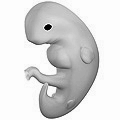
\includegraphics[width=0.2\textwidth]{6_weeks_pregnant.png}}%
\fbox{
\includegraphics[width=0.2\textwidth]{10_weeks_pregnant.png}}%
\fbox{
\includegraphics[width=0.2\textwidth]{20_weeks_pregnant.png}}%
\fbox{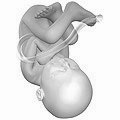
\includegraphics[width=0.2\textwidth]{40_weeks_pregnant.png}}
\end{center}

\begin{center}
\fbox{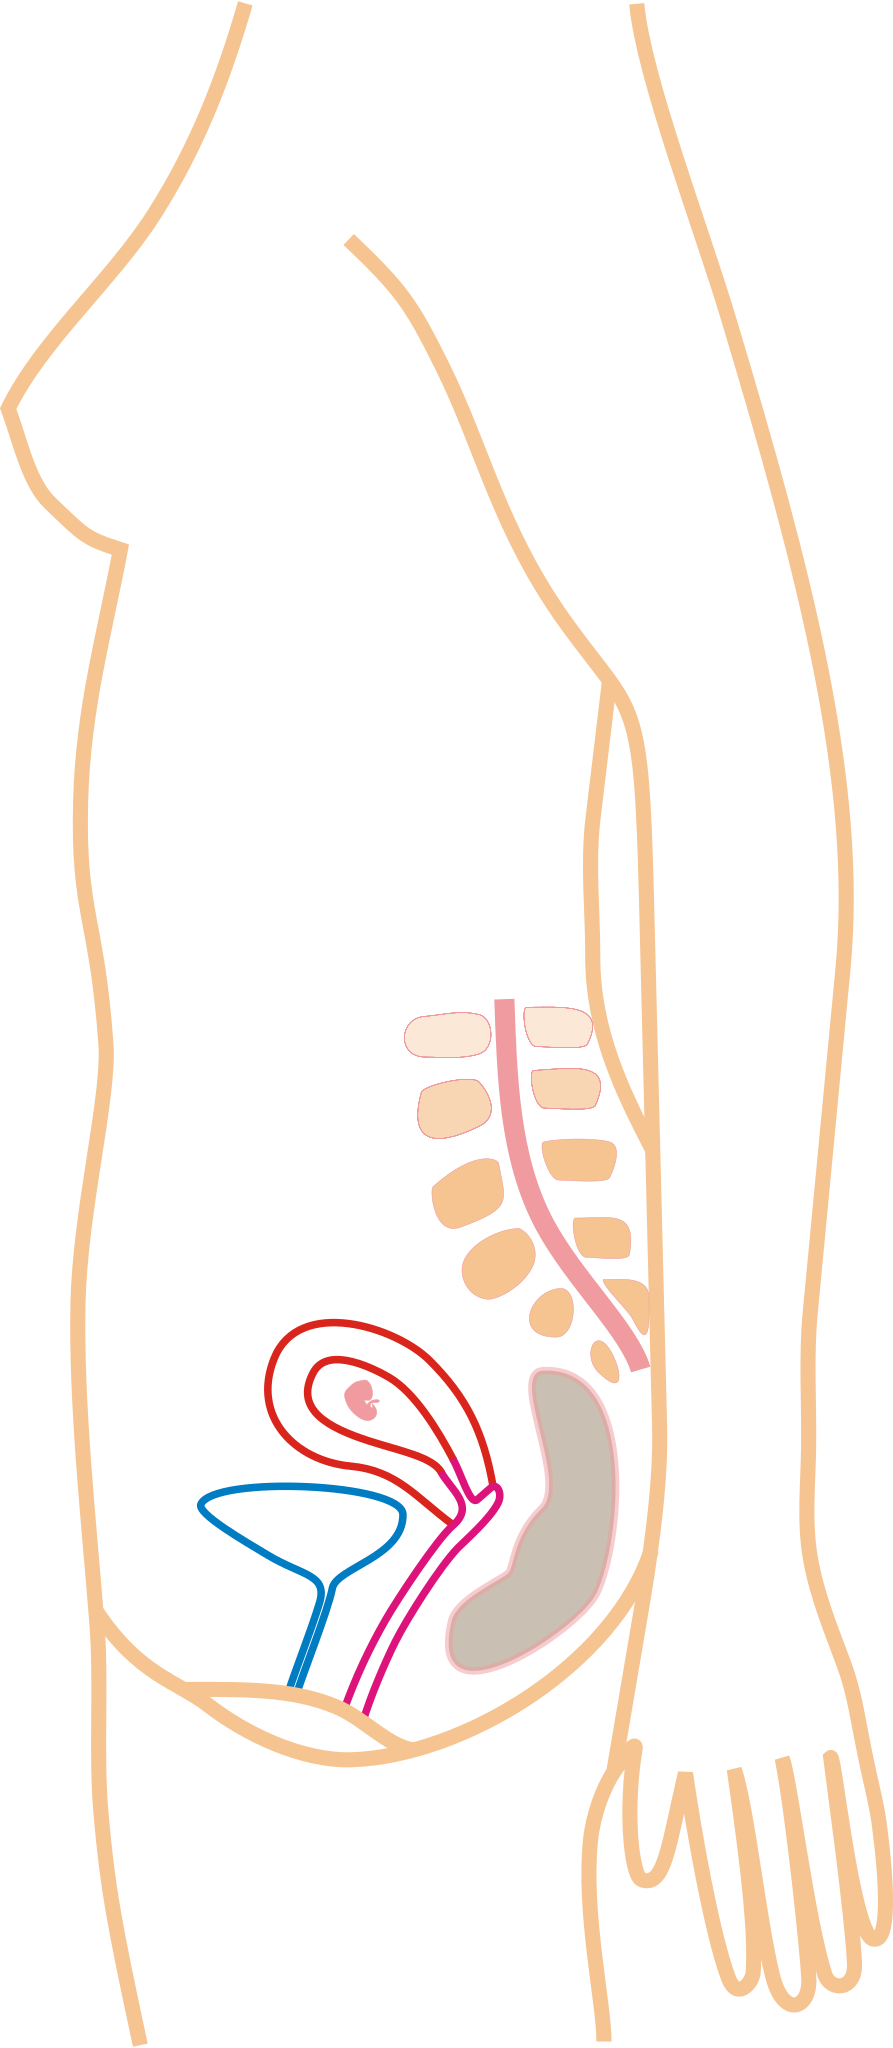
\includegraphics[width=0.2\textwidth,height=0.2\textheight]{Month_1}}%
\fbox{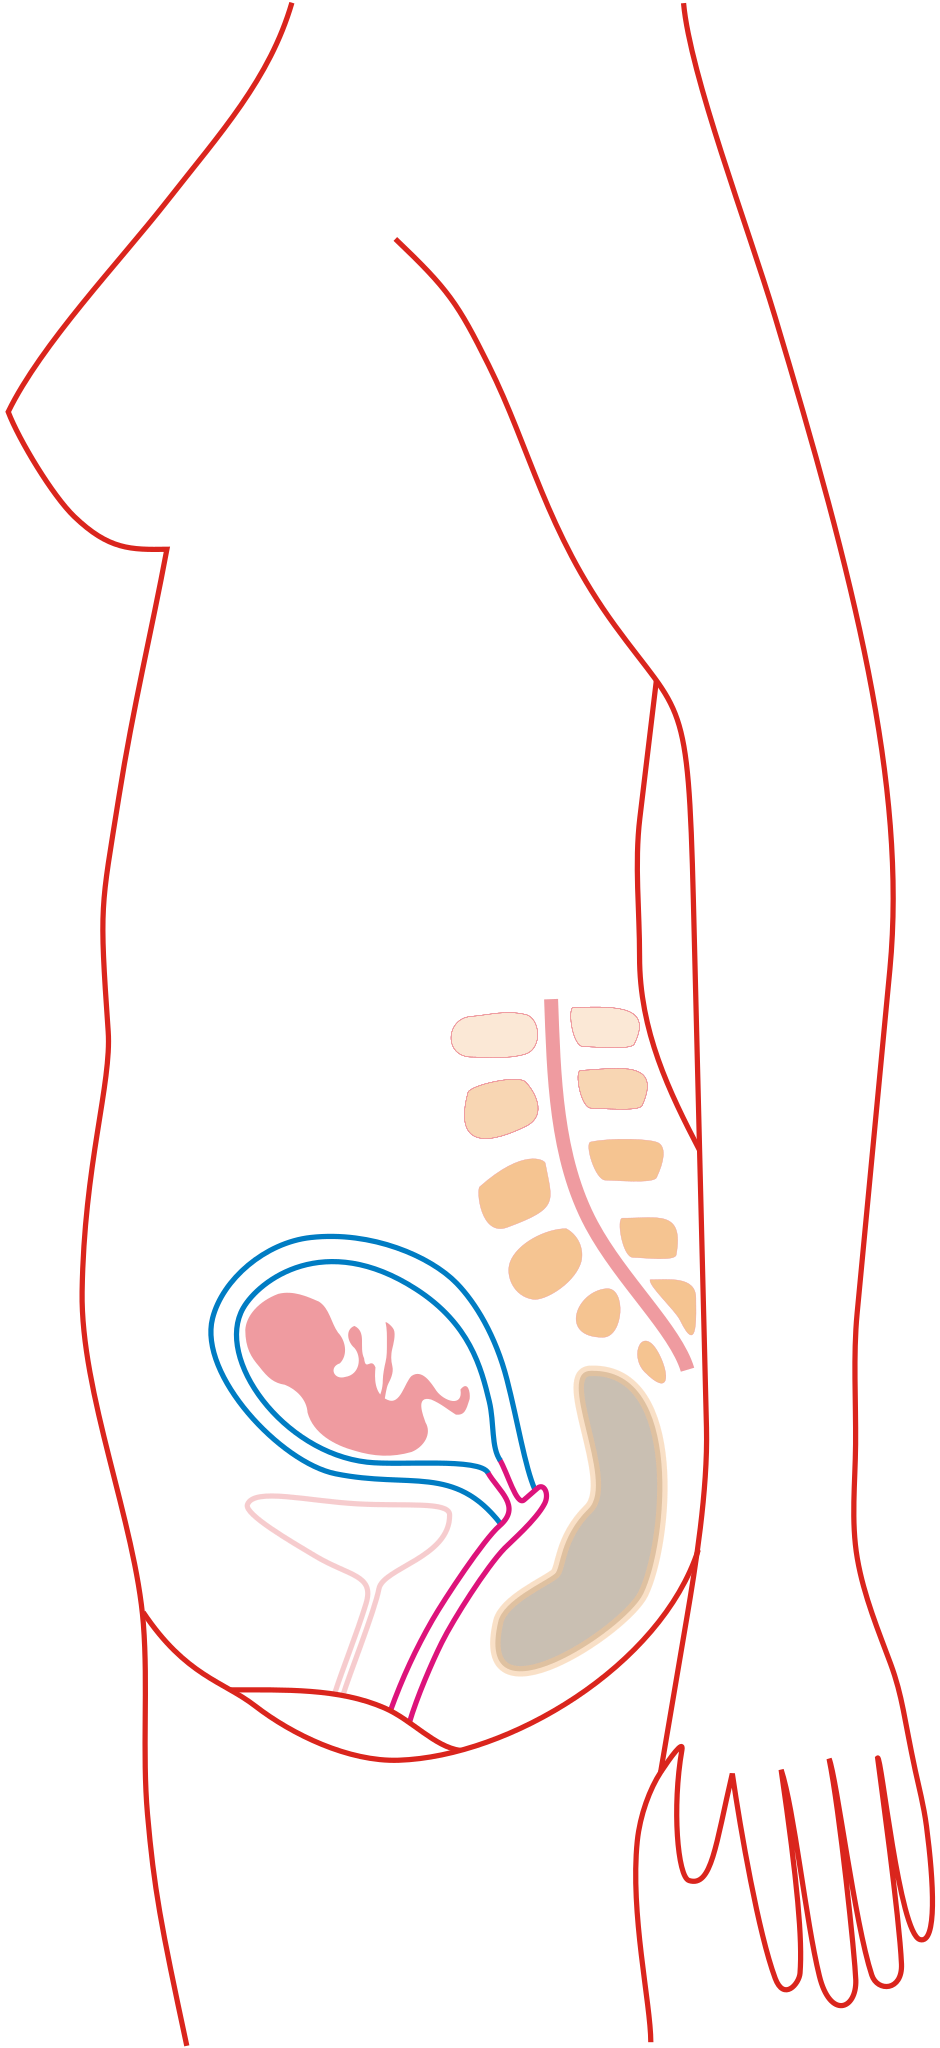
\includegraphics[width=0.2\textwidth,height=0.2\textheight]{Month_3}}%
\fbox{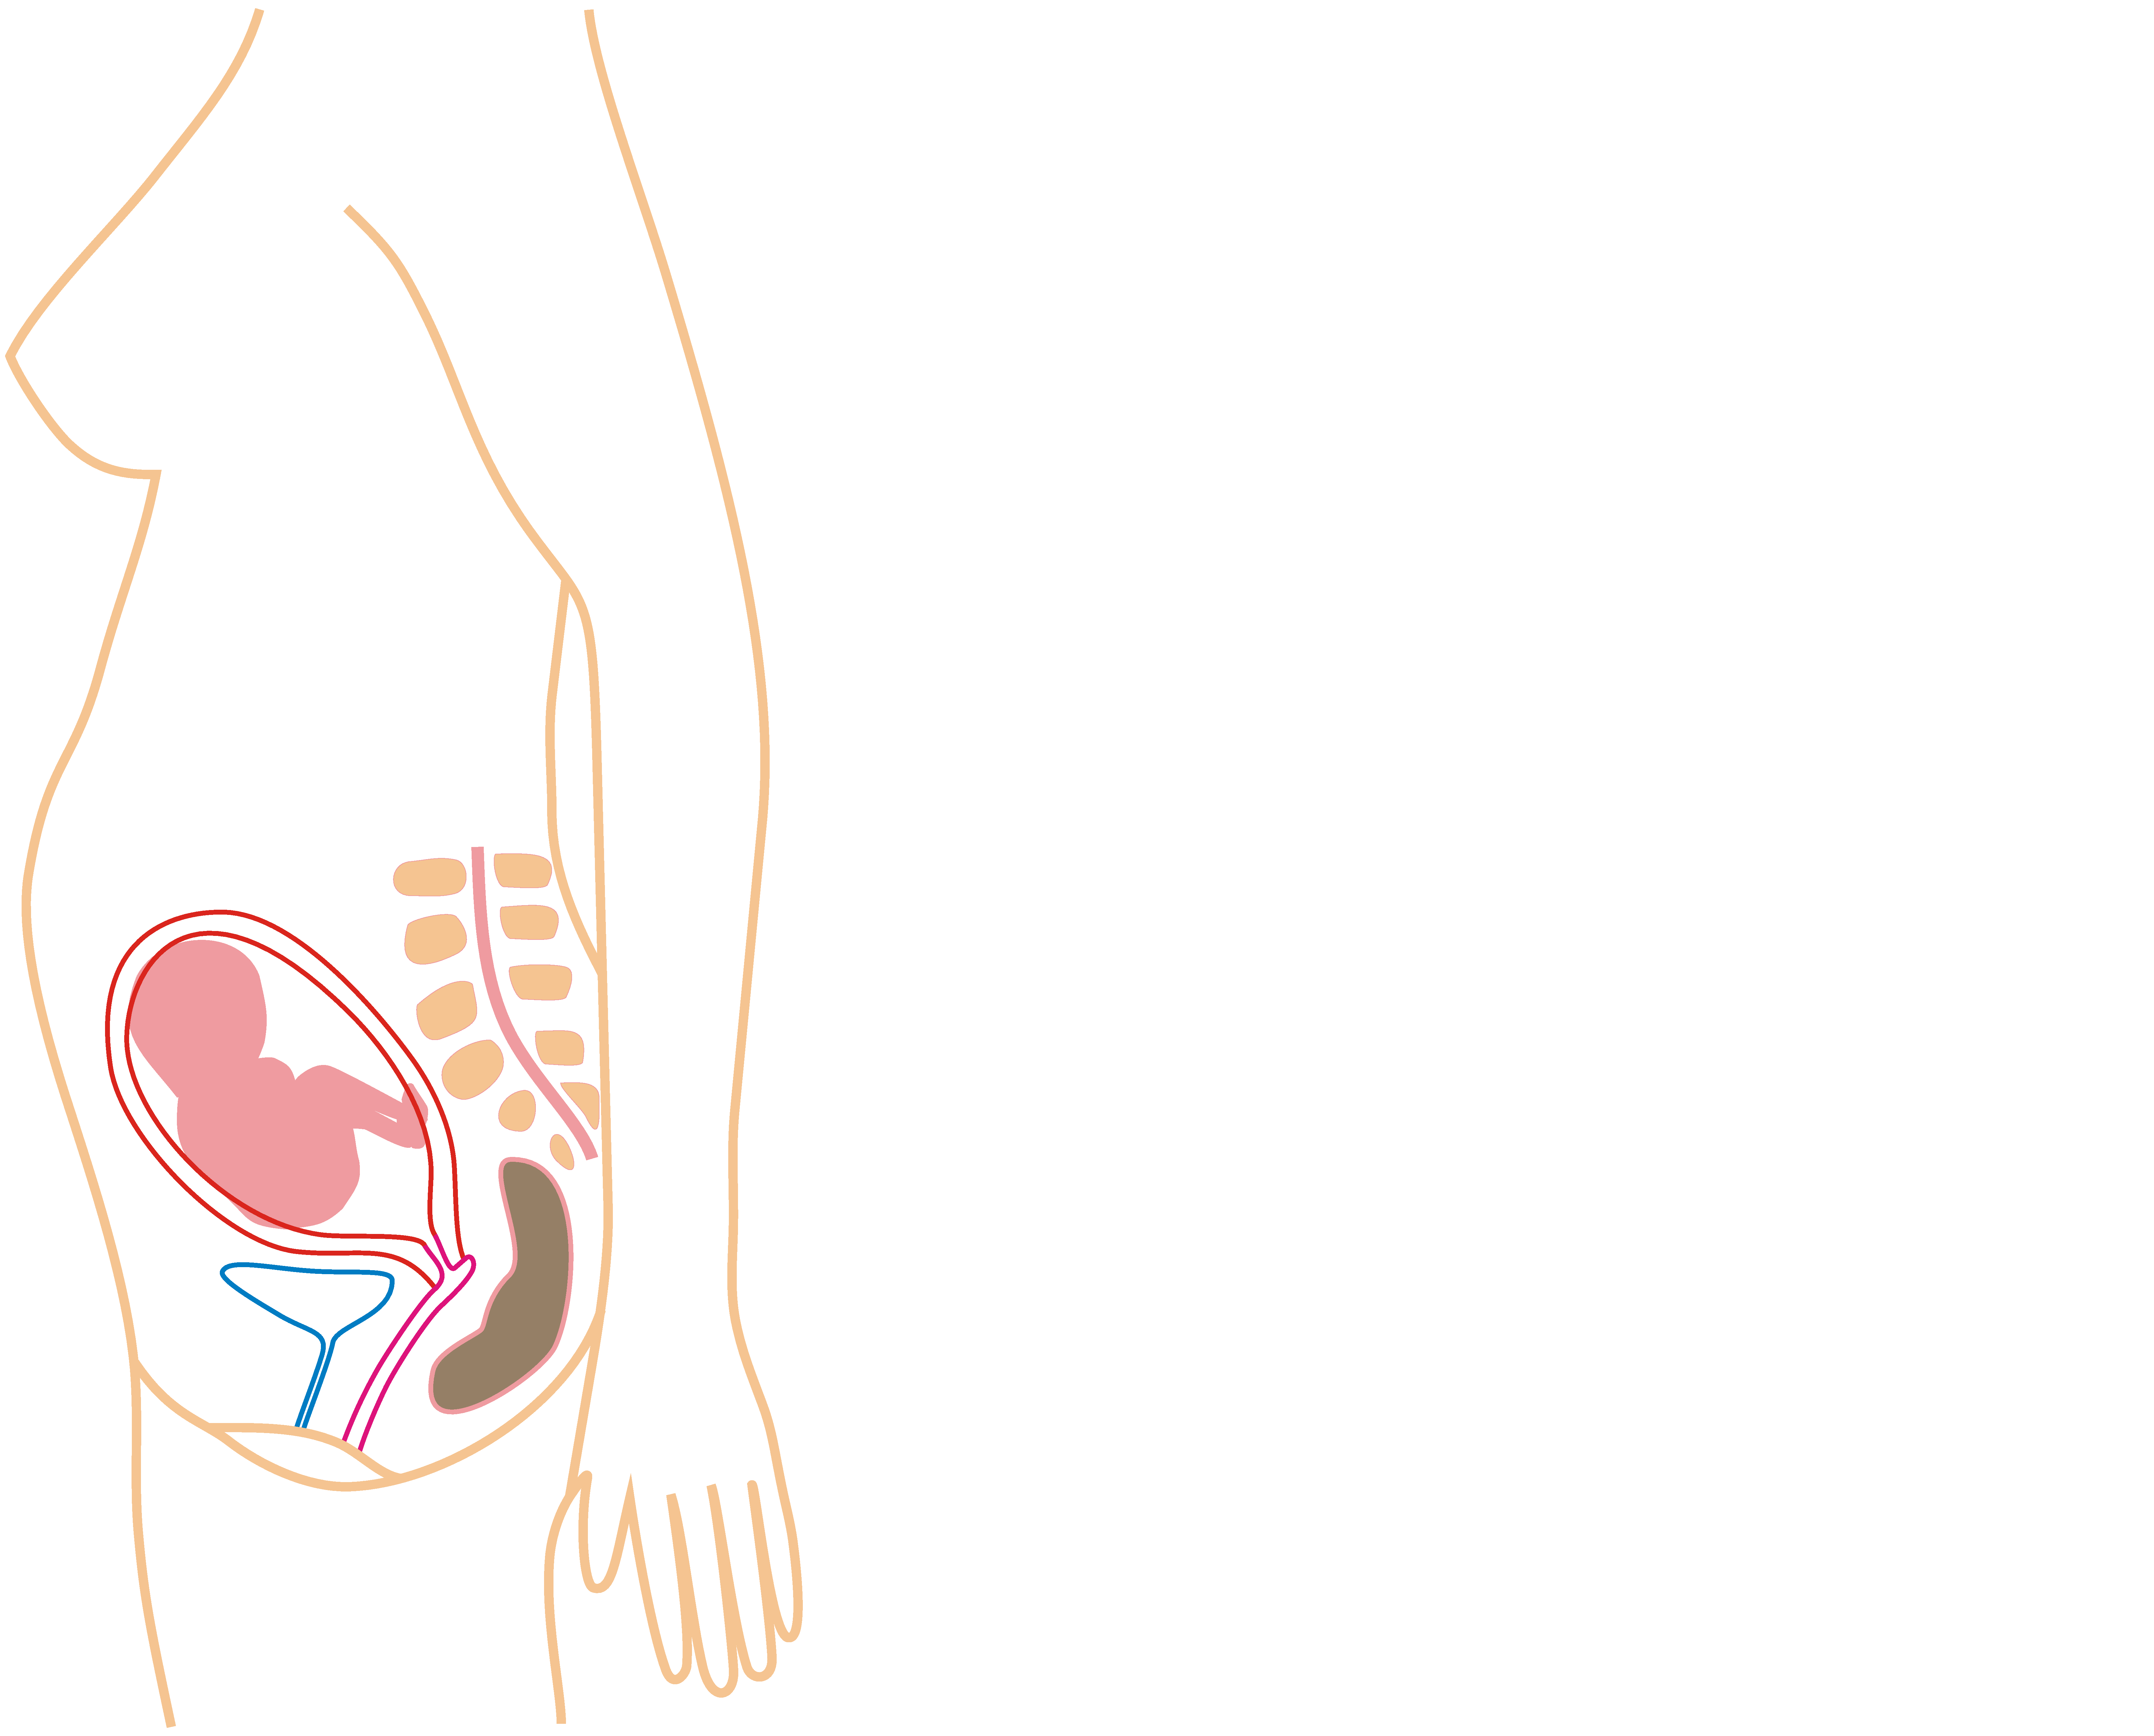
\includegraphics[width=0.2\textwidth,height=0.2\textheight]{Month_5}}%
\fbox{
\includegraphics[width=0.2\textwidth,height=0.2\textheight]{Month_9}}
\end{center}



\section{Physiological changes in pregnancy}

The body must change its physiological and homeostatic mechanisms in pregnancy to ensure the fetus
is provided for. Increases in blood sugar, breathing and cardiac output are all required.

\subsection{Hormonal changes}

Levels of progesterone and oestrogens rise continually throughout pregnancy, suppressing the
hypothalamic axis and subsequently the menstrual cycle. The woman and the placenta also produce many
hormones.

Prolactin levels increase due to maternal Pituitary gland enlargement by 50\%. This mediates a
change in the structure of the Mammary gland from ductal to lobular-alveolar. Parathyroid hormone is
increased due to increases of calcium uptake in the gut and reabsorption by the kidney. Adrenal
hormones such as cortisol and aldosterone also increase.

Placental lactogen is produced by the placenta and stimulates lipolysis and fatty acid metabolism by
the woman, conserving blood glucose for use by the fetus. It also decreases maternal tissue
sensitivity to insulin, resulting in gestational diabetes.

\subsection{Musculoskeletal changes}

The body's posture changes as the pregnancy progresses. The pelvis tilts and the back arches to help
keep balance. Poor posture occurs naturally from the stretching of the woman's abdominal muscles as
the fetus grows. These muscles are less able to contract and keep the lower back in proper
alignment. The pregnant woman has a different pattern of gait. The step lengthens as the pregnancy
progresses, due to weight gain and changes in posture. On average, a woman's foot can grow by a half
size or more during pregnancy. In addition, the increased body weight of pregnancy, fluid retention,
and weight gain lowers the arches of the foot, further adding to the foot's length and width. The
influences of increased hormones such as estrogen and relaxin initiate the remodeling of soft
tissues, cartilage and ligaments. Certain skeletal joints such as the symphysis pubis and sacroiliac
widen or have increased laxity.

\subsection{Physical changes}

One of the most noticeable alterations in pregnancy is the gain in weight. The enlarging uterus, the
growing fetus, the placenta and liquor amnii, the acquisition of fat and water retention, all
contribute to this increase in weight. The weight gain varies from person to person and can be
anywhere from 5 pounds (2.3 kg) to over 100 pounds (45 kg). In America, the doctor-recommended
weight gain range is 25 pounds (11 kg) to 35 pounds (16 kg), less if the woman is overweight, more
(up to 40 pounds (18 kg)) if the woman is underweight.

Other physical changes during pregnancy include breasts increasing two cup sizes. Also areas of the
body such as the forehead and cheeks (known as the 'mask of pregnancy') become darker due to the
increase of melanin being produced.

The female body experiences many changes as the fetus grows through each trimester as shown and
discussed in this pregnancy video. Two women at different stages in their pregnancy illustrate what
has happened to their bodies.

\subsection{Cardiovascular changes}

Blood volume increases by 40\% in the first two trimesters. This is due to an increase in plasma
volume through increased aldosterone. Progesterone may also interact with the aldosterone receptor,
thus leading to increased levels. Red blood cell numbers increase due to increased erythropoietin
levels.

Cardiac function is also modified, with increase heart rate and increased stroke volume. A decrease
in vagal tone and increase in sympathetic tone is the cause. Blood volume increases act to increase
stroke volume of the heart via Starling's law. After pregnancy the change in stroke volume is not
reversed. Cardiac output rises from 4 to 7 litres in the 2nd trimester

Blood pressure also fluctuates. In the first trimester it falls. Initially this is due to decreased
sensitivity to angiotensin and vasodilation provoked by increased blood volume. Later, however, it
is caused by decreased resistance to the growing uteroplacental bed.

\subsection{Respiratory changes}

Decreased functional residual capacity is seen, typically falling from 1.7 to 1.35 litres, due to
the compression of the diaphragm by the uterus. Tidal volume increases, from 0.45 to 0.65 litres,
giving an increase in pulmonary ventilation. This is necessary to meet the increased oxygen
requirement of the body, which reaches 50ml/min - 20ml of which goes to reproductive tissues.

Progesterone may act centrally on chemoreceptors to reset the set point to a lower partial pressure
of carbon dioxide. This maintains an increased respiration rate even at a decreased level of carbon
dioxide.

\subsection{Metabolic changes}

An increased requirement for nutrients is given by fetal growth and fat deposition. Changes are
caused by steroid hormones, lactogen and cortisol.

Maternal insulin resistance can lead to gestational diabetes. Increase liver metabolism is also
seen, with increased gluconeogenesis to increase maternal glucose levels.

\subsection{Renal changes}

Renal plasma flow increases, as does aldosterone and erthropoietin production as discussed. The
tubular maximum for glucose is reduced, which may precipitate gestational diabetes.

\section{Management}

Prenatal medical care is of recognized value throughout the developed world. Periconceptional Folic
acid supplementation is the only type of supplementation of proven efficacy.

\subsection{Nutrition}

A balanced, nutritious diet is an important aspect of a healthy pregnancy. Eating a healthy diet,
balancing carbohydrates, fat, and proteins, and eating a variety of fruits and vegetables, usually
ensures good nutrition. Those whose diets are affected by health issues, religious requirements, or
ethical beliefs may choose to consult a health professional for specific advice.

Adequate periconceptional folic acid (also called folate or Vitamin B9) intake has been proven to
limit fetal neural tube defects, preventing spina bifida, a very serious birth defect. The neural
tube develops during the first 28 days of pregnancy, explaining the necessity to guarantee adequate
periconceptional folate intake. Folates (from folia, leaf) are abundant in spinach (fresh, frozen,
or canned), and are also found in green vegetables, salads, citrus fruit and melon, chickpeas (i.e.
in the form of hummus or falafel), and eggs. In the United States and Canada, most wheat products
(flour, noodles) are fortified with folic acid.

DHA omega-3 is a major structural fatty acid in the brain and retina, and is naturally found in
breast milk. It is important for a mother to consume adequate amounts of DHA during pregnancy and
while nursing to support her well-being and the health of her infant. Developing infants cannot
produce DHA efficiently, and must receive this vital nutrient from the mother through the placenta
during pregnancy and in breast milk after birth.

Several micronutrients are important for the health of the developing fetus, especially in areas of
the world where insufficient nutrition is prevalent. In developed areas, such as Western Europe and
the United States, certain nutrients such as Vitamin D and calcium, required for bone development,
may require supplementation.

Dangerous bacteria or parasites may contaminate foods, particularly listeria and toxoplasma,
toxoplasmosis agent. Careful washing of fruits and raw vegetables may remove these pathogens, as may
thoroughly cooking leftovers, meat, or processed meat. Soft cheeses may contain listeria; if milk is
raw the risk may increase. Cat feces pose a particular risk of toxoplasmosis. Pregnant women are
also more prone to catching salmonella infections from eggs and poultry, which should be thoroughly
cooked. Practicing good hygiene in the kitchen can reduce these risks.

\subsection{Weight gain}

Caloric intake must be increased, to ensure proper development of the fetus. The amount of weight
gained during pregnancy varies among women. The National Health Service recommends that overall
weight gain during the 9 month period for women who start pregnancy with normal weight be 10 to 12
kilograms (22–26 lb). During pregnancy, insufficient weight gain can compromise the health of the
fetus. Women with fears of weight gain or with eating disorders may choose to work with a health
professional, to ensure that pregnancy does not trigger disordered eating. Likewise, excessive
weight gain can pose risks to the woman and the fetus. Women who are prone to being overweight may
choose to plan a healthy diet and exercise to help moderate the amount of weight gained.

\subsection{Immunological tolerance}

Research on the immunological basis for pre-eclampsia has indicated that continued exposure to a
partner's semen has a strong protective effect against pre-eclampsia, largely due to the absorption
of several immune modulating factors present in seminal fluid. Studies also showed that long periods
of sexual cohabitation with the same partner fathering a woman's child significantly decreased her
chances of suffering pre-eclampsia. Several other studies have since investigated the strongly
decreased incidence of pre-eclampsia in women who had received blood transfusions from their
partner, those with long, preceding histories of sex without barrier contraceptives, and in women
who had been regularly performing oral sex, with one study concluding that ``induction of allogeneic
tolerance to the paternal HLA molecules of the fetus may be crucial. Data collected strongly
suggests that exposure, and especially oral exposure to soluble HLA from semen can lead to
transplantation tolerance.''

Other studies have investigated the roles of semen in the female reproductive tracts of mice,
showing that ``insemination elicits inflammatory changes in female reproductive tissues,''
concluding that the changes ``likely lead to immunological priming to paternal antigens or influence
pregnancy outcomes.'' A similar series of studies confirmed the importance of immune modulation in
female mice through the absorption of specific immune factors in semen, including TGF-Beta, lack of
which is also being investigated as a cause of miscarriage in women and infertility in men.

According to the theory, pre-eclampsia is frequently caused by a failure of the woman's immune
system to accept the fetus and placenta, which both contain ``foreign'' proteins from paternal
genes. Regular exposure to the father's semen causes her immune system to develop tolerance to the
paternal antigens, a process which is significantly supported by as many as 93 currently identified
immune regulating factors in seminal fluid. Having already noted the importance of a woman's
immunological tolerance to the fetus's paternal genes, several Dutch reproductive biologists decided
to take their research a step further. Consistent with the fact that human immune systems tolerate
things better when they enter the body via the mouth, the Dutch researchers conducted a series of
studies that confirmed a surprisingly strong correlation between a diminished incidence of
pre-eclampsia and a woman's practice of oral sex, and noted that the protective effects were
strongest if she swallowed her partner's semen. The researchers concluded that while any exposure to
a partner's semen during sexual activity appears to decrease a woman's chances for the various
immunological disorders that can occur during pregnancy, immunological tolerance could be most
quickly established through oral introduction and gastrointestinal absorption of semen. Recognizing
that some of the studies potentially included the presence of confounding factors, such as the
possibility that women who regularly perform oral sex and swallow semen might also engage in more
frequent vaginal intercourse, the researchers also noted that, either way, the data still
overwhelmingly supports the main theory behind all their studies--that repeated exposure to semen
establishes the maternal immunological tolerance necessary for a safe and successful pregnancy.

\subsection{Drugs in pregnancy}

Drugs used during pregnancy can have temporary or permanent effects on the fetus. Therefore many
physicians would prefer not to prescribe for pregnant women, the major concern being over
teratogenicity of the drugs. This results in inappropriate treatment of pregnant women. Use of drugs
in pregnancy is not always wrong. For example, high fever is harmful for the fetus in the early
months. Use of paracetamol is better than no treatment at all. Also, diabetes mellitus during
pregnancy may need intensive therapy with insulin. Drugs have been classified into categories
A,B,C,D and X based on the Food and Drug Administration(FDA) rating system to provide therapeutic
guidance based on potential benefits and fetal risks. Drugs like multivitamins that have
demonstrated no fetal risks after controlled studies in humans are classified as Category A. On the
other hand drugs like thalidomide with proven fetal risks that outweigh all benefits are classified
as Category X.

\subsection{Sexuality during pregnancy}

Most pregnant women can enjoy sexual intercourse throughout gravidity. Most research suggests that,
during pregnancy, both sexual desire and frequency of sexual relations decrease. In context of this
overall decrease in desire, some studies indicate a second-trimester increase, preceding a decrease.
However, these decreases are not universal: a significant number of women report greater sexual
satisfaction throughout their pregnancies.

Sex during pregnancy is a low-risk behaviour except when the physician advises that sexual
intercourse be avoided, because it may, in some pregnancies, lead to serious pregnancy complications
or health issues such as a high-risk for premature labour or a ruptured uterus. Such a decision may
be based upon a history of difficulties in a previous childbirth.

Some psychological research studies in the 1980s and '90s contend that it is useful for pregnant
women to continue to have sexual activity, specifically noting that overall sexual satisfaction was
correlated with feeling happy about being pregnant, feeling more attractive in late pregnancy than
before pregnancy and experiencing orgasm. Sexual activity has also been suggested as a way to
prepare for induced labour; some believe the natural prostaglandin content of seminal liquid can
favour the maturation process of the cervix making it more flexible, allowing for easier and faster
dilation and effacement of the cervix. However, the efficacy of using sexual intercourse as an
induction agent ``remains uncertain''.

During pregnancy, the fetus is protected from penetrative thrusting by the amniotic fluid in the
womb and by the woman's cervix.

After giving birth sexual intercourse can begin when the couple are both ready. However most couples
wait until after six weeks and they should consult their GP if they have any concerns.

\subsection{Abortion}

An abortion is the removal or expulsion of an embryo or fetus from the uterus, resulting in or
caused by its death. This can occur spontaneously or accidentally as with a miscarriage, or be
artificially induced by medical, surgical or other means.


\end{document}
